\documentclass{../zkdl-presentation-template}

\title[Криптографія]{\textbf{Практичне №3.Ентропія. Лінійні регістри зсуву}}

\date{18.09.2025}


\begin{document}
    \frame{
        \titlepage
    }
  
    \begin{frame}{Plan}
        \tableofcontents
    \end{frame}

\section{Ентропія} % Note all sections and subsections are automatically placed in your table of contents

%------------------------------------------------
\begin{frame}
    \frametitle{Визначення ентропії. Повторення}
\begin{block}{}
    Ентропія розподілу ймовірностей $p$:

    \vspace{-9mm}
    \begin{align*}
        p=(p(0),p(1),..,p(n-1)),p(i)\geq 0,i=\overline{1,n},\sum_{i=0}^{n-1}p(i)=1
    \end{align*}

    \vspace{-3mm}
    є числом, яке визначається наступним чином:

    \vspace{-7mm}
    \begin{align*}
        H(p)=-\sum_{i=0}^{n-1}p(i)\cdot\texttt{log}p(i)
    \end{align*}
\end{block}
\begin{alertblock}{}
    Коли виникатиме максимальна ентропія та чому вона буде дорівнювати?
\end{alertblock}

\end{frame}
%------------------------------------------------
\begin{frame}
    \frametitle{Задача}
\begin{block}{}
    Ентропія ансамблю $\langle X,P\rangle$, де $X=\{x_1,x_2,..,x_n\}$, дорівнює $H$. Відбувається «розщеплення» ансамблю: кожен символ $x_i$ замінюється на один з двох символів $\widehat{x_i},\widetilde{x_i}$. Обчисліть ентропію ансамблю $\{\widehat{x_1},\widetilde{x_1},\widehat{x_2},\widetilde{x_2},..,\widehat{x_n},\widetilde{x_n}\}$, якщо $P(\widehat{x_i})=P(\widetilde{x_i})=0,5.$
\end{block}
\begin{figure}
    \centering
    
\includegraphics[width=0.9\linewidth]{2-crypto-sym/images/cells.png}
\end{figure}
\end{frame}

%------------------------------------------------
\begin{frame}
    \frametitle{Задача}
\begin{block}{}
    Риби виду Umbra krameri харчуються переважно дрібними ракоподібними виду Chydorus. З багаторічних досліджень відомо, що ймовірність зустріти у водоймах певного регіону цих риб та рачків одночасно дорівнює $0,25$, не зустріти ні тих, ні інших -- $0,2$, а ймовірність того, що у водоймі є рачки, але немає риб – $0,35$. Нехай подія $А$ -- полягає у тому, що у водоймі є риби, $\overline{A}$ -- що їх немає; відповідно $В$ -- є рачки, $\overline{B}$ -- рачків немає. Знайти взаємну інформацію між ансамблями $А=\{A,\overline{A}\}$, та $B=\{B,\overline{B} \}$
\end{block}
\begin{figure}
    \centering
    
\includegraphics[width=1\linewidth]{2-crypto-sym/images/cells_small.png}
\end{figure}
\end{frame}

%------------------------------------------------
\begin{frame}
    \frametitle{Задача}
\begin{block}{}
    В урні лежать $6$ чорних та $9$ білих кульок. Виймають одну за одною дві кульки випадковим чином без повернення. Нехай $X$ означає колір першої кульки, $Y$ -- другої. Обчислити $H(X), H(Y), H(Y/X)$.
\end{block}
\begin{figure}
    \centering
    
\includegraphics[width=0.9\linewidth]{2-crypto-sym/images/cells.png}
\end{figure}
\end{frame}
%------------------------------------------------
\section{Лінійні регістри зсуву}
%------------------------------------------------
\begin{frame}
    \frametitle{Визначення}
\begin{block}{}
    Лінійний регістр зсуву -- це генератор псевдовипадкової послідовності $\textbf{s}=s_1s_2...s_n$, що задовольняють лінійним рекурентним співвідношенням:
    \vspace{-3mm}
    \begin{align*}
        s_{n+j}=a_0\cdot s_j+a_1\cdot s_{j+1}+...+a_{n-1}\cdot s_{n+j-1}, \quad j=0,1...
    \end{align*}
    
    \vspace{-3mm}
    для фіксованого $n>0$. Коефіцієнти $a_i$, а також члени $s_i$ належать скінченному полю $GF(F_{p^m})$, а операції додавання та множення -- це операції у цьому полі. Такі послідовності називають лінійними рекурентними послідовностями порядку n над скінченним полем $GF(F_{p^m})$. Схематично ЛРЗ можна зобразити таким чином: 
\end{block}
\begin{figure}
    \centering
    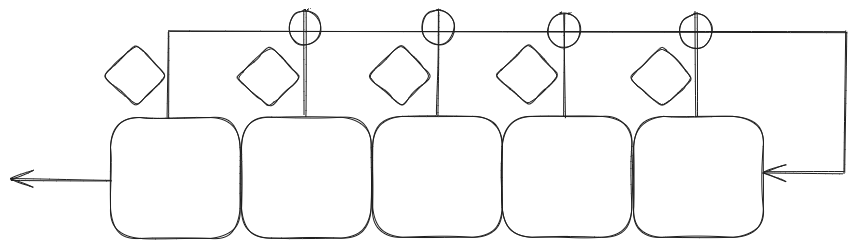
\includegraphics[width=0.65\linewidth]{3-crypto-practice/images/LRZ.png}
\end{figure}
\end{frame}
%------------------------------------------------
\begin{frame}
    \frametitle{Визначення}
\begin{block}{}
    \begin{itemize}
        \item Виходи ЛРЗ формують деяку цикличні послідовність
        \item Для початку роботи задається початковий стан (не нульовий!!!)
    \end{itemize}
\end{block}
\begin{alertblock}{}
    \textbf{Приклад.} Нехай задано поліном виду $x^4+x^3+1$ та поле, над яким задані коефіцієнти $F_2$. Сформуємо рекуренту формулу для обчислення нових станів. Для цього зробимо перетворення степені до індексів $max\_ind=max\_deg$
    \vspace{-3mm}
    \begin{align*}
        x^4+x^3+1=0 \Rightarrow s_4+s_3+s_0=0
    \end{align*}
\end{alertblock}
\begin{figure}
    \centering
    
\includegraphics[width=0.9\linewidth]{2-crypto-sym/images/cells_small.png}
\end{figure}
\end{frame}
%------------------------------------------------




    \begin{frame}[plain, standout]
    \begin{figure}
        \centering
        
\includegraphics[width=0.9\linewidth]{Cryptocats.jpg}
        \label{fig:placeholder}
    \end{figure}
    \centering
    \LARGE
    \textbf{Питання?} \\

    \vspace{0.2cm} \Huge \ding{170} \large \\

  \end{frame}
\end{document}